\section{Decision Trees}
\begin{frame}{The ML Toolbox: Roadmap Update}
    \centering \vspace*{\fill} \hspace*{-0.6cm}
    \resizebox{1.1\linewidth}{!}{
    \begin{tikzpicture}[node distance=0.5cm, box/.style={scale=1.25, rectangle, draw=gray!40, fill=gray!5, rounded corners, minimum width=2.8cm, minimum height=1.8cm, align=center, font=\small}, active/.style={draw=myblue, fill=blue!10, line width=1.5pt}, completed/.style={draw=mygreen, fill=green!10, line width=1pt, dashed}, arrow/.style={-latex, thick, gray!60}]
        \node[font=\bfseries\Large] (root) at (0, 3) {Machine Learning Models ($f_\theta$)};
        \node[box, completed] (linear) at (-6, 0) {\textbf{1. Linear Models}};
        \node[box, completed] (distance) at (-2, 0) {\textbf{2. Distance-Based}};
        \node[box, completed] (kernel) at (2, 0) {\textbf{3. Kernel-Based}};
        \node[box, active] (trees) at (6, 0) {\textbf{4. Tree-Based}\\Decision Trees,\\Forests \& GBM};
        \draw[arrow] (root) -- (linear); \draw[arrow] (root) -- (distance); \draw[arrow] (root) -- (kernel); \draw[arrow] (root) -- (trees);
        \node[myblue, below=0.3cm of trees, font=\bfseries] {$\uparrow$ We Are Here};
    \end{tikzpicture}
    } \vspace*{\fill}
\end{frame}

% --- Slide 1: Decision Tree Intuition (Fixed & Titanic Theme) ---
\begin{frame}{Decision Trees}
    \textbf{Intuition:} We split data by asking a sequence of Yes/No questions to separate classes.
    \vspace{0.5em}

    \begin{columns}[c]
        \begin{column}{0.5\textwidth}
            \centering
            % Tree Visual - Fixed sibling distance to prevent overlap
            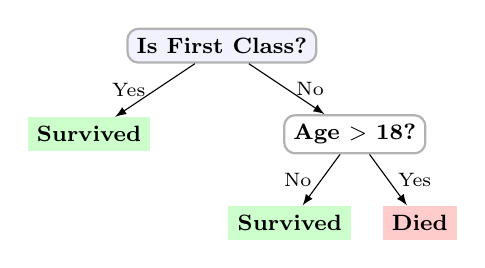
\begin{tikzpicture}[
            scale=0.75,
                level distance=1.5cm,
                level 1/.style={sibling distance=4.5cm}, % Increased width
                level 2/.style={sibling distance=2.2cm}, % Increased width
                node/.style={rectangle, draw=gray!60, rounded corners, fill=white, font=\footnotesize, align=center, thick},
                leaf_survived/.style={rectangle, draw=none, fill=green!20, font=\bfseries\footnotesize},
                leaf_died/.style={rectangle, draw=none, fill=red!20, font=\bfseries\footnotesize},
                edge from parent/.style={draw, -latex}
            ]
              
              \node[node, fill=blue!5] {\textbf{Is First Class?}}
                child {node[leaf_survived] {Survived} 
                    edge from parent node[left, font=\scriptsize] {Yes}
                }
                child {node[node] {\textbf{Age $>$ 18?}} 
                    child {node[leaf_survived] {Survived} 
                        edge from parent node[left, font=\scriptsize] {No}
                    }
                    child {node[leaf_died] {Died} 
                        edge from parent node[right, font=\scriptsize] {Yes}
                    }
                    edge from parent node[right, font=\scriptsize] {No}
                };
            \end{tikzpicture}
        \end{column}
        
        \begin{column}{0.5\textwidth}
            \textbf{Example: Titanic Survival}
            \begin{itemize}
                \item \textbf{Goal:} Predict who survived.
                \item \textbf{Root Question:} "Was the passenger in First Class?" (Best separator).
                \item \textbf{Next Question:} If not, "Were they a child?"
            \end{itemize}

            \pause
            \vspace{1em}
            \begin{alertblock}{\centering The Core Question}
                \centering
                We have many features (Age, Ticket, Gender...). \\
                \textbf{How do we decide which question to ask first?}
            \end{alertblock}
        \end{column}
    \end{columns}
\end{frame}

% --- Slide 2: Impurity Metrics (Added p_i definition) ---
\begin{frame}{How to Choose the Best Split? (Purity)}
    We want questions that lead to \textbf{"Pure" nodes} (containing only one class).
    We measure "disorder" using \textbf{Impurity Metrics}.

    \vspace{0.5em}
    \begin{columns}[T]
        \begin{column}{0.45\textwidth}
            \centering
            \textbf{Visualizing Impurity}
            \vspace{0.5em}
            
            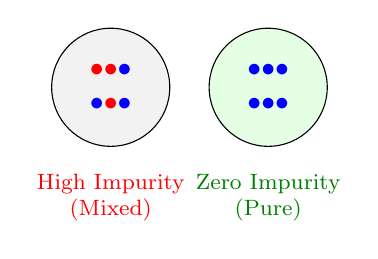
\begin{tikzpicture}[scale=1.0]
                % Impure Node
                \node[circle, draw, minimum size=1.5cm, fill=gray!10, align=center] at (0,0) {
                    \textcolor{red}{$\bullet$}\textcolor{red}{$\bullet$}\textcolor{blue}{$\bullet$}\\
                    \textcolor{blue}{$\bullet$}\textcolor{red}{$\bullet$}\textcolor{blue}{$\bullet$}
                };
                \node[font=\footnotesize, red, align=center] at (0, -1.4) {High Impurity\\(Mixed)};

                % Pure Node
                \node[circle, draw, minimum size=1.5cm, fill=green!10, align=center] at (2,0) {
                    \textcolor{blue}{$\bullet$}\textcolor{blue}{$\bullet$}\textcolor{blue}{$\bullet$}\\
                    \textcolor{blue}{$\bullet$}\textcolor{blue}{$\bullet$}\textcolor{blue}{$\bullet$}
                };
                \node[font=\footnotesize, green!50!black, align=center] at (2, -1.4) {Zero Impurity\\(Pure)};
            \end{tikzpicture}

            \vspace{1em}
    \centering
    \small \textbf{The Algorithm's Goal:} Pick the split that maximizes the drop in Impurity (Information Gain).
    
        \end{column}
        
        \begin{column}{0.55\textwidth}
            \textbf{The "Impurity Metrics":}
            \small
            \begin{enumerate}
                \item \textbf{Gini Impurity (Default):}
                $$ G = 1 - \sum p_i^2 $$
                \vspace{-3mm}
                \small
                \begin{itemize}
                    \item $G=0.5$: Max chaos (50/50).
                    \item $G=0.0$: Pure (One class).
                \end{itemize}
                \item \textbf{Entropy (Information):}
                $$ H = - \sum p_i \log_2(p_i) $$
            \end{enumerate}
            
            % \vspace{0.5em}
            \begin{tcolorbox}[colback=yellow!10, colframe=orange!40, boxsep=2pt, left=2pt, right=2pt, top=2pt, bottom=2pt]
                \centering
                \textbf{What is $p_i$?} \\
                $p_i$ is the \textbf{proportion} of samples belonging to class $i$ in the current node.
            \end{tcolorbox}
        \end{column}
    \end{columns}
\end{frame}
% --- Slide: Optimization Method (Trees vs Linear) ---
\begin{frame}{Wait... Where is Gradient Descent?}
    \textbf{Q:} Do Decision Trees use Gradient Descent to find the best split?
    \pause
    
    \begin{alertblock}{The Answer: NO!}
        Standard Decision Trees are \textbf{Non-Differentiable}.
        You cannot calculate a gradient $\nabla J$ because splits are discrete "hard" choices (Left vs. Right).
    \end{alertblock}
    
\end{frame}

\begin{frame}{Wait... Where is Gradient Descent?}
    \textbf{Comparison of Learning Algorithms:}

    \begin{columns}[T]
        \begin{column}{0.50\textwidth}
            \begin{tcolorbox}[colback=blue!5, title=\textbf{Non-Trees Models}]
                \textbf{Method:} Gradient Descent
                \begin{itemize}
                    \item Loss surface is smooth (convex).
                    \item We slide down the curve.
                    \item Update weights $\mathbf{w}$ iteratively.
                \end{itemize}
            \end{tcolorbox}
        \end{column}
        
        \begin{column}{0.55\textwidth}
            \begin{tcolorbox}[colback=green!5, title=\textbf{Decision Trees}]
                \textbf{Method:} Greedy Search
                \begin{itemize}
                    \item Try \textbf{every possible split} for every feature.
                    \item Pick the one with max Information Gain.
                    \item {\textbf{Repeat recursively until:}
            \begin{itemize}
                \item The node is \textbf{Pure} (100\% one class).
                \item Or we hit a \textbf{Stop Condition} (e.g., Max Depth).
            \end{itemize}}
                \end{itemize}
            \end{tcolorbox}
        \end{column}
    \end{columns}
    
\end{frame}

% --- Slide 8: Decision Trees Pros/Cons ---
\begin{frame}{Decision Trees: Advantages and Disadvantages}
    \begin{columns}[T]
        \begin{column}{0.48\textwidth}
            \begin{tcolorbox}[colback=green!5, title=\textbf{The Advantages}]
                \small
                \begin{itemize}
                    \item \textbf{Simple:} Easy to understand.
                    \item \textbf{Interpretable:} Easy to explain to non-experts ("If X $>$ 5, then Y").
                    \item \textbf{No Preprocessing Required:} No feature scaling or encoding required.
                
                \end{itemize}
            \end{tcolorbox}
        \end{column}
        \begin{column}{0.48\textwidth}
            \begin{tcolorbox}[colback=red!5, title=\textbf{The Disadvantages}]
                \small
                \begin{itemize}
                    \item \textbf{High Variance:} A small change in data = completely different tree.
                    \item \textbf{Overfitting:} Not setting the stop conditions (e.g., Max Depth) guarantees overfitting.
                \end{itemize}
            \end{tcolorbox}
        \end{column}
    \end{columns}
\end{frame}

% --- Slide 9: Random Forest (Bagging) ---
